% Options for packages loaded elsewhere
% Options for packages loaded elsewhere
\PassOptionsToPackage{unicode}{hyperref}
\PassOptionsToPackage{hyphens}{url}
%
\documentclass[
  ignorenonframetext,
  aspectratio=169,
  russian,
]{beamer}
\newif\ifbibliography
\usepackage{pgfpages}
\setbeamertemplate{caption}[numbered]
\setbeamertemplate{caption label separator}{: }
\setbeamercolor{caption name}{fg=normal text.fg}
\beamertemplatenavigationsymbolshorizontal
% remove section numbering
\setbeamertemplate{part page}{
  \centering
  \begin{beamercolorbox}[sep=16pt,center]{part title}
    \usebeamerfont{part title}\insertpart\par
  \end{beamercolorbox}
}
\setbeamertemplate{section page}{
  \centering
  \begin{beamercolorbox}[sep=12pt,center]{section title}
    \usebeamerfont{section title}\insertsection\par
  \end{beamercolorbox}
}
\setbeamertemplate{subsection page}{
  \centering
  \begin{beamercolorbox}[sep=8pt,center]{subsection title}
    \usebeamerfont{subsection title}\insertsubsection\par
  \end{beamercolorbox}
}
% Prevent slide breaks in the middle of a paragraph
\widowpenalties 1 10000
\raggedbottom
\AtBeginPart{
  \frame{\partpage}
}
\AtBeginSection{
  \ifbibliography
  \else
    \frame{\sectionpage}
  \fi
}
\AtBeginSubsection{
  \frame{\subsectionpage}
}
\usepackage{iftex}
\ifPDFTeX
  \usepackage[T1]{fontenc}
  \usepackage[utf8]{inputenc}
  \usepackage{textcomp} % provide euro and other symbols
\else % if luatex or xetex
  \usepackage{unicode-math} % this also loads fontspec
  \defaultfontfeatures{Scale=MatchLowercase}
  \defaultfontfeatures[\rmfamily]{Ligatures=TeX,Scale=1}
\fi
\usepackage{lmodern}

\ifPDFTeX\else
  % xetex/luatex font selection
\fi
% Use upquote if available, for straight quotes in verbatim environments
\IfFileExists{upquote.sty}{\usepackage{upquote}}{}
\IfFileExists{microtype.sty}{% use microtype if available
  \usepackage[]{microtype}
  \UseMicrotypeSet[protrusion]{basicmath} % disable protrusion for tt fonts
}{}


\usepackage{longtable,booktabs,array}
\newcounter{none} % for unnumbered tables
\usepackage{calc} % for calculating minipage widths
\usepackage{caption}
% Make caption package work with longtable
\makeatletter
\def\fnum@table{\tablename~\thetable}
\makeatother
\usepackage{graphicx}
\makeatletter
\newsavebox\pandoc@box
\newcommand*\pandocbounded[1]{% scales image to fit in text height/width
  \sbox\pandoc@box{#1}%
  \Gscale@div\@tempa{\textheight}{\dimexpr\ht\pandoc@box+\dp\pandoc@box\relax}%
  \Gscale@div\@tempb{\linewidth}{\wd\pandoc@box}%
  \ifdim\@tempb\p@<\@tempa\p@\let\@tempa\@tempb\fi% select the smaller of both
  \ifdim\@tempa\p@<\p@\scalebox{\@tempa}{\usebox\pandoc@box}%
  \else\usebox{\pandoc@box}%
  \fi%
}
% Set default figure placement to htbp
\def\fps@figure{htbp}
\makeatother



\ifLuaTeX
\usepackage[bidi=basic,shorthands=off,provide=*]{babel}
\else
\usepackage[bidi=default,shorthands=off,provide=*]{babel}
\fi
\ifLuaTeX
  \usepackage{selnolig} % disable illegal ligatures
\fi


\setlength{\emergencystretch}{3em} % prevent overfull lines

\providecommand{\tightlist}{%
  \setlength{\itemsep}{0pt}\setlength{\parskip}{0pt}}



 

\usepackage[]{csquotes}

\IfFileExists{plex-otf.sty}{
  %% Full TeXlive
  % \usepackage[%
  %   % math,
  %   RM={Scale=0.94},SS={Scale=0.94},SScon={Scale=0.94},TT={Scale=MatchLowercase,FakeStretch=0.9},DefaultFeatures={Ligatures=Common}
  % ]{plex-otf}
}{
  %% TinyTeX
  \usepackage{libertine}
}

%%% Load theme
% https://deic.uab.cat/~iblanes/beamer_gallery/
\IfFileExists{beamerthemegotham.sty}{
  %% Full TeXlive
  \usetheme{gotham}
  \gothamset{
    numbering=totalpagenumber,
    parttocframe default=off,
    sectiontocframe default=off,
    subsectiontocframe default=off,
  }
}{
  %% TinyTeX
  \usetheme{Madrid}
}
\makeatletter
\@ifpackageloaded{caption}{}{\usepackage{caption}}
\AtBeginDocument{%
\ifdefined\contentsname
  \renewcommand*\contentsname{Содержание}
\else
  \newcommand\contentsname{Содержание}
\fi
\ifdefined\listfigurename
  \renewcommand*\listfigurename{Список иллюстраций}
\else
  \newcommand\listfigurename{Список иллюстраций}
\fi
\ifdefined\listtablename
  \renewcommand*\listtablename{Список таблиц}
\else
  \newcommand\listtablename{Список таблиц}
\fi
\ifdefined\figurename
  \renewcommand*\figurename{Рисунок}
\else
  \newcommand\figurename{Рисунок}
\fi
\ifdefined\tablename
  \renewcommand*\tablename{Таблица}
\else
  \newcommand\tablename{Таблица}
\fi
}
\@ifpackageloaded{float}{}{\usepackage{float}}
\floatstyle{ruled}
\@ifundefined{c@chapter}{\newfloat{codelisting}{h}{lop}}{\newfloat{codelisting}{h}{lop}[chapter]}
\floatname{codelisting}{Список}
\newcommand*\listoflistings{\listof{codelisting}{Листинги}}
\makeatother
\makeatletter
\makeatother
\makeatletter
\@ifpackageloaded{caption}{}{\usepackage{caption}}
\@ifpackageloaded{subcaption}{}{\usepackage{subcaption}}
\makeatother

\usepackage{bookmark}
\IfFileExists{xurl.sty}{\usepackage{xurl}}{} % add URL line breaks if available
\urlstyle{same}
% fallback for those not using the hyperref driver hyperxmp:
\makeatletter
\@ifundefined{xmpquote}{\newcommand{\xmpquote}[1]{#1}}{}
\makeatother
\hypersetup{
  pdftitle={Лабораторная работа №5},
  pdfauthor={Кудякова София Андреевна},
  pdflang={ru},
  hidelinks,
  pdfcreator={LaTeX via pandoc}}


\title{\texorpdfstring{Лабораторная работа №5}{Лабораторная работа №5}}
\subtitle{\texorpdfstring{Аппарат сетей Петри}{Аппарат сетей Петри}}
\author{Кудякова София Андреевна}
\date{2026-08-29}

\begin{document}
\frame{\titlepage}

\renewcommand*\contentsname{Содержание}
\begin{frame}[allowframebreaks]
  \frametitle{Содержание}
  \setcounter{tocdepth}{1}
  \tableofcontents
\end{frame}
\setcounter{tocdepth}{1}
\tableofcontents
}

\section{Введение}\label{ux432ux432ux435ux434ux435ux43dux438ux435}

\begin{frame}{Цель и задачи}
\protect\phantomsection\label{ux446ux435ux43bux44c-ux438-ux437ux430ux434ux430ux447ux438}
\textbf{Цель:} изучить аппарат сетей Петри на примере задачи «Обедающие
философы».

\textbf{Задачи:}

\begin{itemize}[<+->]
\tightlist
\item
  построить классическую сеть Петри и исследовать deadlock;
\item
  реализовать модифицированную сеть с арбитром;
\item
  выполнить стохастическое (Гиллеспи) и детерминированное моделирование;
\item
  построить анимацию и провести сравнительный анализ;
\item
  реализовать литературное программирование и получить
  Julia/Notebook/Quarto.
\end{itemize}
\end{frame}

\begin{frame}{Сети Петри}
\protect\phantomsection\label{ux441ux435ux442ux438-ux43fux435ux442ux440ux438}
Сеть Петри задаётся четвёркой:

\[
N = (P, T, F, M_0)
\]

\begin{itemize}[<+->]
\tightlist
\item
  \(P\) --- позиции (состояния/ресурсы);
\item
  \(T\) --- переходы (события);
\item
  \(F\) --- дуги между позициями и переходами;
\item
  \(M_0\) --- начальная маркировка.
\end{itemize}

Смена маркировки происходит при срабатывании разрешённого перехода.
\end{frame}

\begin{frame}[fragile]{Задача «Обедающие философы»}
\protect\phantomsection\label{ux437ux430ux434ux430ux447ux430-ux43eux431ux435ux434ux430ux44eux449ux438ux435-ux444ux438ux43bux43eux441ux43eux444ux44b}
\(N\) философов и \(N\) вилок за круглым столом. Состояния философа:

\begin{itemize}[<+->]
\tightlist
\item
  \texttt{Think} --- размышляет;
\item
  \texttt{Hungry} --- голоден;
\item
  \texttt{Eat} --- ест (нужны обе соседние вилки).
\end{itemize}

Каждая вилка --- общий ресурс, недоступный одновременно двум философам.
\end{frame}

\begin{frame}[fragile]{Deadlock и арбитр}
\protect\phantomsection\label{deadlock-ux438-ux430ux440ux431ux438ux442ux440}
Если все философы одновременно захватят левую вилку, каждый будет ждать
правую --- \textbf{взаимная блокировка (deadlock)}.

Для предотвращения вводится позиция \texttt{Arbiter} с \(N-1\) фишками
--- не позволяет всем \(N\) философам одновременно начать захват вилок.
\end{frame}

\section{Реализация}\label{ux440ux435ux430ux43bux438ux437ux430ux446ux438ux44f}

\begin{frame}[fragile]{Структура проекта}
\protect\phantomsection\label{ux441ux442ux440ux443ux43aux442ux443ux440ux430-ux43fux440ux43eux435ux43aux442ux430}
Проект \texttt{lab05} на DrWatson: \texttt{src}, \texttt{scripts},
\texttt{data}, \texttt{plots}, \texttt{notebooks}, \texttt{report}.

Основной модуль: \texttt{src/DiningPhilosophers.jl} со структурой
\texttt{PetriNet} (позиции, переходы, матрица инцидентности).
\end{frame}

\begin{frame}[fragile]{Классическая сеть и сеть с арбитром}
\protect\phantomsection\label{ux43aux43bux430ux441ux441ux438ux447ux435ux441ux43aux430ux44f-ux441ux435ux442ux44c-ux438-ux441ux435ux442ux44c-ux441-ux430ux440ux431ux438ux442ux440ux43eux43c}
Каждый философ: позиции \texttt{Think\_i}, \texttt{Hungry\_i},
\texttt{Eat\_i}, \texttt{Fork\_i}.

При \(N=5\): \(4N=20\) позиций, \(3N=15\) переходов.

\begin{itemize}[<+->]
\tightlist
\item
  \textbf{Классическая сеть:} \texttt{Think} → \texttt{Hungry} (захват
  левой вилки) → попытка захватить правую → \texttt{Eat} → возврат
  вилок.
\item
  \textbf{Сеть с арбитром:} добавлена позиция \texttt{Arbiter} с
  начальной маркировкой \(N-1=4\) --- разрешение арбитра обязательно для
  захвата ресурса.
\end{itemize}
\end{frame}

\section{Моделирование}\label{ux43cux43eux434ux435ux43bux438ux440ux43eux432ux430ux43dux438ux435}

\begin{frame}{Стохастическое моделирование (алгоритм Гиллеспи)}
\protect\phantomsection\label{ux441ux442ux43eux445ux430ux441ux442ux438ux447ux435ux441ux43aux43eux435-ux43cux43eux434ux435ux43bux438ux440ux43eux432ux430ux43dux438ux435-ux430ux43bux433ux43eux440ux438ux442ux43c-ux433ux438ux43bux43bux435ux441ux43fux438}
Шаг алгоритма: расчёт интенсивностей → время до события → выбор перехода
→ изменение маркировки → сохранение состояния.

Параметры эксперимента: \(N=5\), \(t_{\max}=50\).
\end{frame}

\begin{frame}[fragile]{Классическая сеть --- результат}
\protect\phantomsection\label{ux43aux43bux430ux441ux441ux438ux447ux435ux441ux43aux430ux44f-ux441ux435ux442ux44c-ux440ux435ux437ux443ux43bux44cux442ux430ux442}
Автоматическая проверка \texttt{detect\_deadlock}: для классической сети
ожидается переход в состояние без дальнейших изменений.

\begin{figure}

\centering{


\includegraphics[width=0.75\linewidth,height=\textheight,keepaspectratio]{image/1.png}

}

\caption{\label{fig-classic}Динамика состояний позиций классической
сети}

\end{figure}%
\end{frame}

\begin{frame}[fragile]{Сеть с арбитром --- результат}
\protect\phantomsection\label{ux441ux435ux442ux44c-ux441-ux430ux440ux431ux438ux442ux440ux43eux43c-ux440ux435ux437ux443ux43bux44cux442ux430ux442}
Для сети с арбитром \texttt{detect\_deadlock} должен возвращать
\texttt{false}.

\begin{figure}

\centering{


\includegraphics[width=0.75\linewidth,height=\textheight,keepaspectratio]{image/2.png}

}

\caption{\label{fig-arbiter}Изменение состояний философов в сети с
арбитром}

\end{figure}%
\end{frame}

\begin{frame}[fragile]{Детерминированное моделирование}
\protect\phantomsection\label{ux434ux435ux442ux435ux440ux43cux438ux43dux438ux440ux43eux432ux430ux43dux43dux43eux435-ux43cux43eux434ux435ux43bux438ux440ux43eux432ux430ux43dux438ux435}
Система ОДУ строится по матрице инцидентности сети
(\texttt{simulate\_ode}), решается методом \texttt{Tsit5}.

\begin{figure}

\centering{


\includegraphics[width=0.75\linewidth,height=\textheight,keepaspectratio]{image/3.png}

}

\caption{\label{fig-ode}Динамика маркировки при детерминированном
моделировании}

\end{figure}%
\end{frame}

\section{Анимация}\label{ux430ux43dux438ux43cux430ux446ux438ux44f}

\begin{frame}[fragile]{Визуализация динамики}
\protect\phantomsection\label{ux432ux438ux437ux443ux430ux43bux438ux437ux430ux446ux438ux44f-ux434ux438ux43dux430ux43cux438ux43aux438}
Уменьшенная модель: \(N=3\), \(t_{\max}=30\). Результат --- GIF-анимация
\texttt{philosophers\_simulation.gif}, наблюдается перемещение фишек
между \texttt{Think}, \texttt{Hungry}, \texttt{Eat}, \texttt{Fork}.

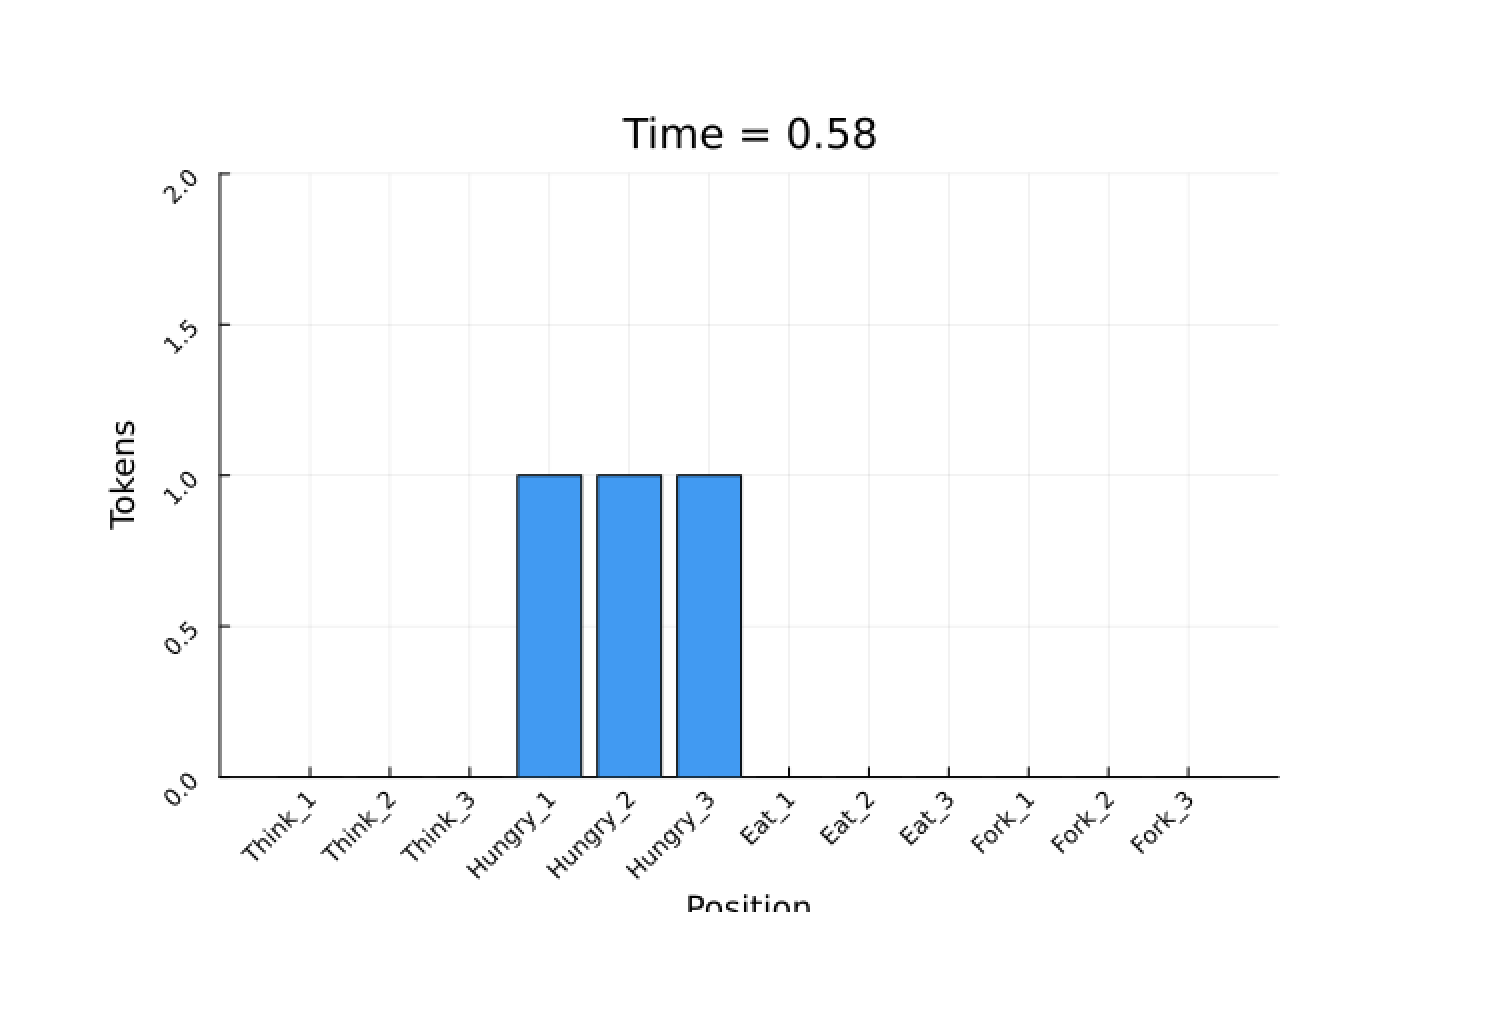
\includegraphics[width=0.45\linewidth,height=\textheight,keepaspectratio,alt={Кадр анимации}]{image/401.png}

\includegraphics[width=0.45\linewidth,height=\textheight,keepaspectratio,alt={Кадр анимации}]{image/44.png}
\end{frame}

\begin{frame}{Кадры анимации (продолжение)}
\protect\phantomsection\label{ux43aux430ux434ux440ux44b-ux430ux43dux438ux43cux430ux446ux438ux438-ux43fux440ux43eux434ux43eux43bux436ux435ux43dux438ux435}

\includegraphics[width=0.45\linewidth,height=\textheight,keepaspectratio,alt={Кадр анимации}]{image/444.png}
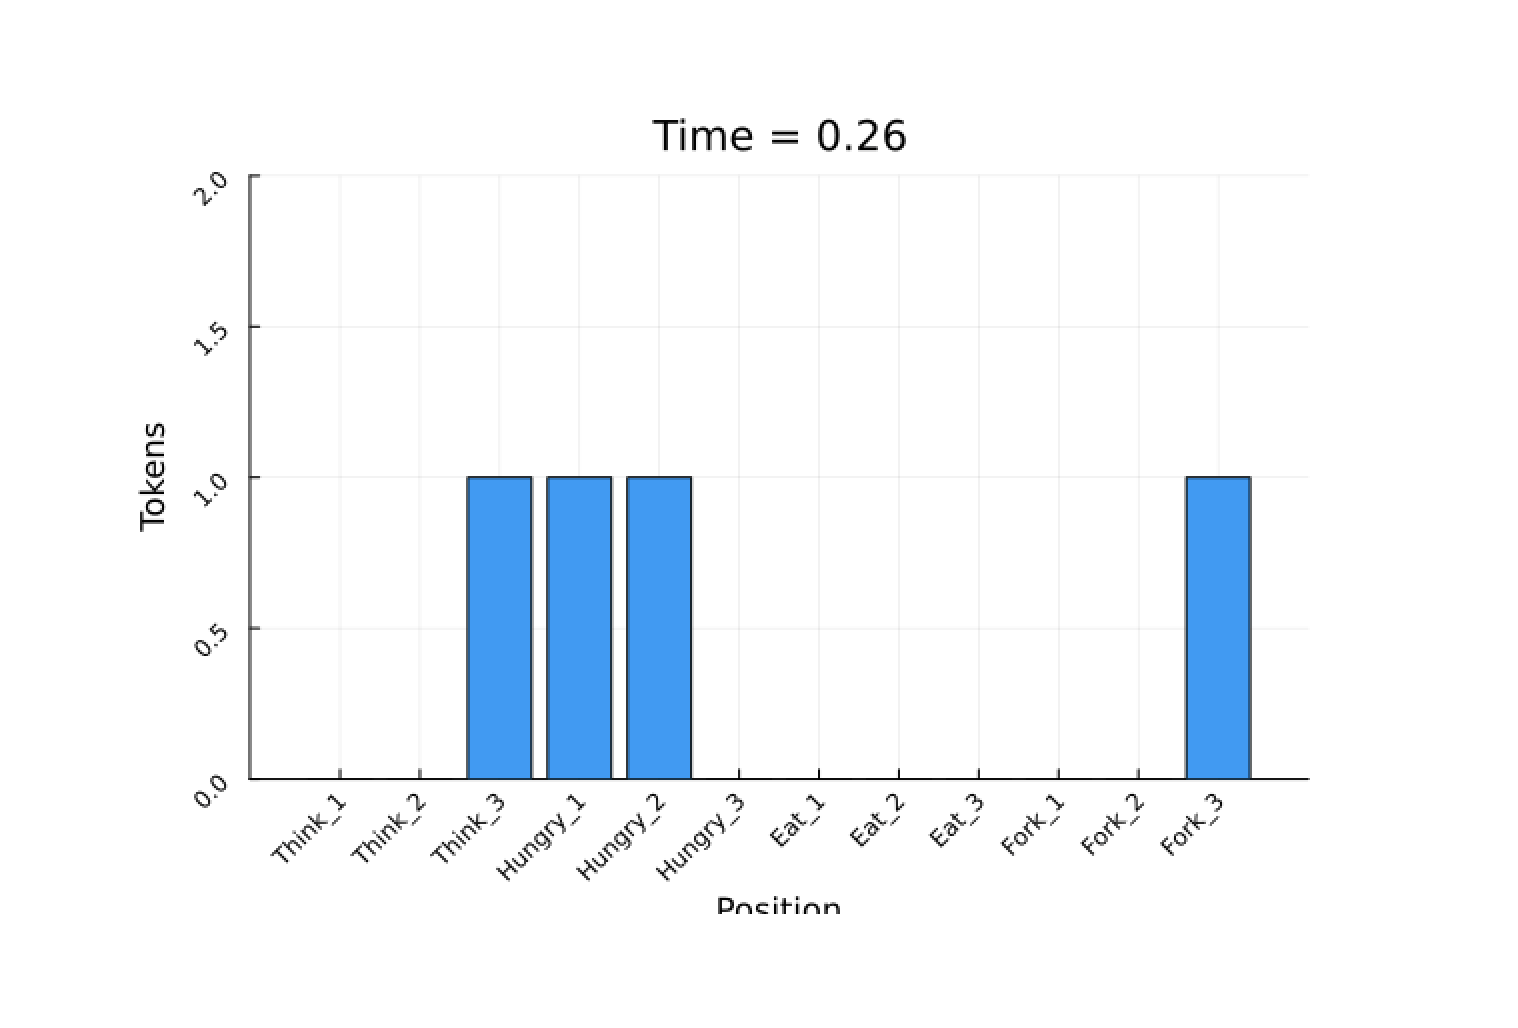
\includegraphics[width=0.45\linewidth,height=\textheight,keepaspectratio,alt={Кадр анимации}]{image/104.png}
\end{frame}

\section{Сравнение и литературное
программирование}\label{ux441ux440ux430ux432ux43dux435ux43dux438ux435-ux438-ux43bux438ux442ux435ux440ux430ux442ux443ux440ux43dux43eux435-ux43fux440ux43eux433ux440ux430ux43cux43cux438ux440ux43eux432ux430ux43dux438ux435}

\begin{frame}[fragile]{Сравнительный анализ}
\protect\phantomsection\label{ux441ux440ux430ux432ux43dux438ux442ux435ux43bux44cux43dux44bux439-ux430ux43dux430ux43bux438ux437}
Скрипт \texttt{dining\_philosophers\_report.jl} сравнивает состояние
\texttt{Eat\_i} классической сети и сети с арбитром.

\begin{figure}

\centering{


\includegraphics[width=0.75\linewidth,height=\textheight,keepaspectratio]{image/5.png}

}

\caption{\label{fig-comparison}Сравнение динамики Eat\_i для
классической сети и сети с арбитром}

\end{figure}%

В классической сети \texttt{Eat\_i} перестаёт изменяться после deadlock;
в сети с арбитром --- продолжает изменяться.
\end{frame}

\begin{frame}[fragile]{Литературное программирование}
\protect\phantomsection\label{ux43bux438ux442ux435ux440ux430ux442ux443ux440ux43dux43eux435-ux43fux440ux43eux433ux440ux430ux43cux43cux438ux440ux43eux432ux430ux43dux438ux435}
Файл \texttt{dining\_philosophers\_literate.jl} объединяет текст и код.
Через \texttt{Literate.jl} получены: Julia-скрипт, Quarto-документ
(\texttt{QuartoFlavor}), Jupyter Notebook.

\begin{figure}

\centering{


\includegraphics[width=0.75\linewidth,height=\textheight,keepaspectratio]{image/6.png}

}

\caption{\label{fig-literate}Литературный исходный файл модели}

\end{figure}%
\end{frame}

\begin{frame}{Jupyter Notebook}
\protect\phantomsection\label{jupyter-notebook}
Сгенерированный ноутбук выполнен в Jupyter, проверены ячейки и
результаты.

\begin{figure}

\centering{


\includegraphics[width=0.75\linewidth,height=\textheight,keepaspectratio]{image/7.png}

}

\caption{\label{fig-jupyter}Выполненный Jupyter Notebook}

\end{figure}%
\end{frame}

\section{Результаты}\label{ux440ux435ux437ux443ux43bux44cux442ux430ux442ux44b}

\begin{frame}[fragile]{Анализ}
\protect\phantomsection\label{ux430ux43dux430ux43bux438ux437}
\begin{itemize}[<+->]
\tightlist
\item
  классическая сеть демонстрирует взаимную блокировку;
\item
  арбитр с \(N-1\) разрешениями предотвращает deadlock;
\item
  сравнение \texttt{Eat\_i} подтверждает разницу в поведении моделей.
\end{itemize}
\end{frame}

\begin{frame}[fragile]{Выводы}
\protect\phantomsection\label{ux432ux44bux432ux43eux434ux44b}
\begin{itemize}[<+->]
\tightlist
\item
  реализована структура \texttt{PetriNet}, классическая и
  модифицированная модели;
\item
  выполнено стохастическое (Гиллеспи) и детерминированное (ОДУ)
  моделирование;
\item
  создана анимация и проведён сравнительный анализ;
\item
  реализовано литературное программирование: Julia-скрипт, Quarto,
  Jupyter Notebook.
\end{itemize}
\end{frame}




\end{document}
